\documentclass{beamer}

% chktex-file 1
% chktex-file 8

\usetheme[workplace=fi]{MU}
\usepackage[utf8]{inputenc}
\usepackage[
  main=czech,
  english
]{babel}
\usepackage[utf8]{inputenc}
\usepackage[T1]{fontenc}
\usepackage{csquotes}
\usepackage{booktabs}
\usepackage{amsmath}

\usepackage{graphicx}


\title{Comparing subtelomeric sequences in human genomes in terms
    of sequence (and methylation) similarity}
\author{Jindřich Matuška}
\institute[FI MU]{Faculty of Informatics, Masaryk University}
\date{\today}

\begin{document}

\frame{\titlepage}

\title{Comparing subtelomeric sequences in human genomes}

\frame{%
    \frametitle{Subtelomeres}

    \begin{itemize}
        \item Region ca. 500000 bp beside telomeres
        \item Frequent modifications
        \item Transposable element
    \end{itemize}
    }

\frame{%
    \frametitle{Why do that}

    \begin{itemize}
        \item Modifications (duplication) may lead to:
            \begin{itemize}
                \item creation of new genes
                \item diversification of chromosomes
            \end{itemize}
    \end{itemize}
}

\frame{%
    \frametitle{Pipeline}

    \begin{enumerate}
        \item Extraction of subtelomeres
        \item Similiarity by ModDotPlot
        \item Further analysis
    \end{enumerate}
}

\frame{%
    \frametitle{Extraction of subtelomeres}

    \begin{enumerate}
        \item Extraction of buffered sequence from ends (SeqKit, script)
        \item Extraction of telomere regions (Seqtk telo)
        \item Inversion, cropping subtelomeres to length (bedtools, script, SeqKit)
        \item Reversion of end sequences (SeqKit)
    \end{enumerate}
}

\frame{
    \frametitle{Similiarity by ModDotPlot}

    \begin{enumerate}
        \item Selection of subtelomeres (SeqKit)
        \item Split by N-sequences (script, SeqKit)
        \item Sort, merge (SeqKit)
        \item Similiarity analysis (ModDotPlot)
        \item Finish?
    \end{enumerate}
}

\frame{
    \frametitle{Further analysis}

    \begin{enumerate}
        \item Parsing .bedpe files into heatmap (Python, Matplotlib)  % chktex 26
        \item Selection of groups (SeqKit)
        \item Similiarity analysis (ModDotPlot)
    \end{enumerate}
}

\frame{
    \frametitle{Running pipeline}

    2 slow parts

    \begin{itemize}
        \item Extraction of buffered sequences from ends
        \item ModDotPlot
    \end{itemize}

    Otherwise quite fast
}

\frame{
    \frametitle{Analysis of heatmap}

    3 groups with high similiarity:

    \begin{itemize}
        \item Big tandem repeats
        \item Singleton chr21-A
        \item Small similiar subsequences
    \end{itemize}
}

\frame{
    \phantom{}\vspace{-4em}
    \begin{centering}
        \begin{figure}
            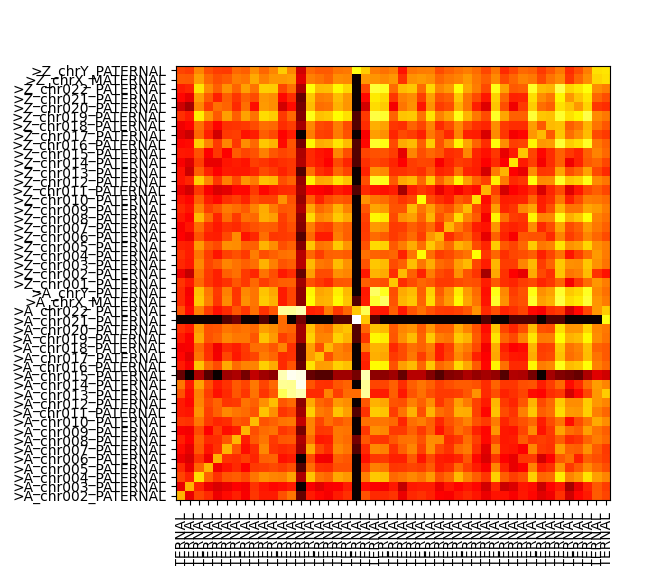
\includegraphics[width=\textwidth]{resources/full_hist.png}
        \end{figure}
    \end{centering}
}

\frame{
    \frametitle{Groups}

    Big tandem repeats

    \begin{itemize}
        \item chr13-A
        \item chr14-A
        \item chr15-A
        \item chr22-A
    \end{itemize}

    Singleton chr21-A
}

\frame{
    \phantom{}\vspace{-4em}
    \begin{centering}
        \begin{figure}
            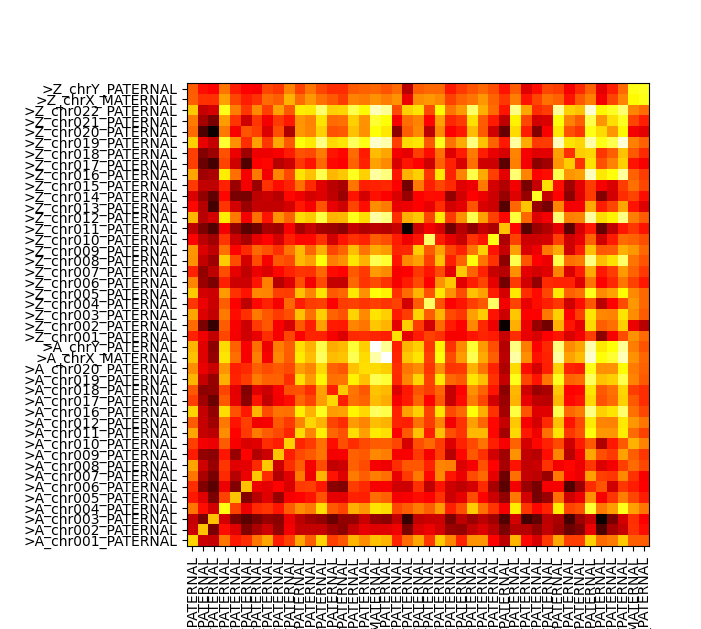
\includegraphics[width=\textwidth]{resources/wo_large.png}
        \end{figure}
    \end{centering}
}

\frame{
    \frametitle{Groups 2}

    Small similiar subsequences

    \begin{itemize}
        \item chr16-A
        \item chrX-A
        \item chrY-A
        \item chr8-Z
        \item chr12-Z
        \item chr16-Z
        \item chr19-Z
        \item chr20-Z
        \item chr22-Z
    \end{itemize}
}

\frame{
    \frametitle{Further work}

    \begin{itemize}
        \item Extraction of sequences
        \item Methylation data
        \item Multiple sources of data
    \end{itemize}
}

\end{document}
